\input{../common}

\begin{document}
  %<*content>
  \lesson{analysis}{25}{ La fonction exponentielle }
  
Combien de grains de sable faudrait-il pour remplir l'univers ?

C'est à partir de cette question qu'Archimède définit le premier, au III\up{e} siècle avant J.C, un phénomène que nous qualifions aujourd'hui  d'exponentiel.

Toute fois c'est Leonhard Euler  (1707- 1784)  qui donna son nom à cette fonction et qui la relia à des phénomènes temporels.


C'est aujourd'hui  une fonction que l'on retrouve dans tous les domaines de la modélisation, que ce soit pour prévoir l'évolution d'une population, comprendre la trajectoire d'une particule etc.

Par exemple une chaîne de lettres demande à la personne qui la reçoit de copier la lettre et de l'envoyer à quatre autres personnes. Supposant que personne ne brise la chaîne, dresser un tableau de valeurs qui montre le nombre de lettres dans la chaîne à chaque stade, à six stades. La situation  peut-être  représentée une fonction exponentielle. \\


 $  \begin{array}{lrcl}
 \text{La fonction }\;\;  \ln  : & \intoo{0}{\pinf}  &   \longrightarrow &  \Rr \\ 
  &  x & \longmapsto & \ln x \; \; \text{est bijective}
  
 \end{array}$ \\
 Elle admet donc  une bijection  réciproque  de  $\; \Rr \;$  vers $\;  \intoo{0}{\pinf} $.
 
 
\subsection{Définition et propriétés}


\begin{definition}
 On appelle fonction exponentielle,  notée $ \exp$,  la bijection réciproque de la fonction logarithme népérien.
\end{definition}

\begin{center}

   $  \begin{array}{lrcl}
 \text{On a donc}\qquad \exp  : & \Rr  &   \longrightarrow &  \intoo{0}{\pinf} \\ 
  &  x & \longmapsto & \exp(x)  \end{array} $ 
\end{center}

\begin{notation}
Pour tout  $ x $  réel quelconque, le nombre $ \exp(x) $ se  note   $\; \eexp{x},\;$ ce qui se lit << $ \mathrm{e} $  puissance $ x $>>. 
\[\boxed{\exp(x)=\eexp{x}}\quad \text{où}\;\mathrm{e}\; \text{est le nombre d'Euler étudié dans la leçon sur la fonction }\;\ln. \]
\end{notation}
\begin{example} [ calcul à l'aide  de la calculatrice]

$$\begin{array}{|c|c|c|c|c|c|c|c|c|c|c|}
\hline
 x & -3&  -1 &  0 &  0.2  &0.5 &  1 &  2  &  8  &  10  & 15 \\
\hline
 \eexp{x}    & 0,049  & 0,36 & 1 & 1,22 & 1,64 & 2,718& 7,38 &2980,95 &22026,46 &3269017,37\\
\hline

\end{array}$$


\end{example}
\begin{corollary}
\begin{itemize}
\item[\textbullet] Pour tout  \; $ x \in \Rr,\; \; \eexp{x}> 0 $

\item[\textbullet] $  \eexp{0}= 1 $  
\item[\textbullet] $ \eexp{1}= \mathrm{e} $

 \item[\textbullet]  Pour tout \; $ x> 0,\; \; \eexp{\ln x}=x  $
 
 
  \item[\textbullet]   Pour tout\;  $ y\in \Rr ,\; \; \ln (\eexp{y})=y  $
  
  
   \item[\textbullet] $ \exp $  est continue et dérivable sur  $ \Rr $.
  
  \end{itemize}

\end{corollary}

\fbox{$\text{Pour  tout réel  } \; X \; \text{strictement positif}\;\; \ln X=Y\; \text{si et seulement si} \; X=\eexp{Y}.$}
\begin{property}
La fonction $ \exp $  est  strictement croissante  sur $ \Rr $.

\begin{itemize}
 \item[\textbullet] $ \eexp{a}=\eexp{b}\; \text{équivaut à }\;  a=b $
   \item[\textbullet] $ \eexp{a}> \eexp{b}  \; \text{équivaut à }\;  a>b $
   \end{itemize}
\end{property}
\begin{property}
Pour tous $ a $ et $ b $  réels:

\begin{itemize}
\item[\textbullet] $\eexp{a+b} =\eexp{a}\eexp{b} $
\item[\textbullet] $ \eexp{a-b }=\dfrac{\eexp{a}}{\eexp{b} }$
\item[\textbullet] $ \eexp{-a }=\dfrac{1}{\eexp{a} }$
\item[\textbullet] $ \paren{\eexp{a }}^{r}= \eexp{ra }$,\quad $  r\in\Qq $
\end{itemize}
\end{property}

\begin{example}
\begin{itemize}
\item[\textbullet] $\eexp{x}\paren{1+2\eexp{-x}} =\eexp{x}+2\eexp{x}\eexp{-x}=\eexp{x}+2$
\item[\textbullet] $ \dfrac{\eexp{2x}}{\eexp{3x}}=\eexp{2x-3x}=\eexp{-x}$
\item[\textbullet] $ \dfrac{\eexp{x+2}}{\eexp{x+1}} =\eexp{(x+2)-(x+1)}=\eexp{1}=\eexp{}$
\item[\textbullet] $ \paren{\eexp{x}+\eexp{-x}}^{2}=\paren{\eexp{x}}^{2} +2\times \eexp{x}\eexp{-x}+\paren{\eexp{-x}}^{2}=\eexp{2x}+2+\eexp{-2x}$
\end{itemize}
\end{example}

\subsection{Étude et représentation graphique}
\begin{property}[Dérivée]
 La fonction exponentielle est dérivable sur $ \Rr $ et est égale à sa propre dérivée:\\
 
 $ \paren{ \eexp{x}}^{\prime}=\eexp{x}  \quad$ pour tout  $\; x \in \Rr $

\end{property}


\textbf{Limites}\\
Aux bornes de l'ensemble de définition de la fonction exp, on obtient les limites suivantes:



\begin{property}
$ \bullet \;\displaystyle \lim_{x \to \pinf}\eexp{x} =\pinf \hspace*{2cm} \bullet \;   \displaystyle\lim_{x \to \minf}\eexp{ x}=0 $

\end{property}

\textbf{Tableau de variation}
\begin{center}
\begin{tikzpicture}
\tkzTab[lgt=2]
{
	$x$ / 0.5 ,
	$\exp^{\prime}(x)$ / 0.5,
	$\exp(x)$ /1
}
{ $\minf$ , $\pinf$ }
{ , + , }
{-/ $0$ , +/$\pinf$ }
\end{tikzpicture}


\end{center}

La droite d'équation $ y=0 $  c'est-à-dire l'axe des abscisses est une asymptote à la courbe de la fonction $ \exp$  en $ \minf $.\\
\textbf{Représentation graphique de la fonction exp}\\
Les  courbes de la fonction  $ \exp $  et de la fonction $ \ln  $ sont symétriques  par  rapport à la première bissectrice du repère.
  \begin{center}
\begin{tikzpicture}[>=stealth', scale=0.5]
\clip (-4,-3) rectangle (7,7);
\draw[->,thick] (0,0) -- (1,0);
\draw[->,thick] (0,0) -- (0,1);
\draw[,thick] (-4,0) -- (7,0);
\draw[thick] (0,-3) -- (0,7);
\foreach\x in {1,2,}
{
\draw[thick] (\x,0.1) -- (\x,-0.1) node[below] {\x};
}
\foreach\y in {1}
{
\draw[thick] (0.1,\y) -- (-0.1,\y) node[left] {\y};
}

\draw[thick,black] plot[domain=0.1 :7,samples=100] (\x,{ln (\x)}) node[above left] {$\mathscr{C_{\ln}}$};
\draw[thick,black] plot[domain=-3 :1.78,samples=100] (\x,{exp (\x)}) node[above left] {$\mathscr{C_{\exp}}$};
\draw[thick,dashed] plot[domain=-3 :7,samples=100] (\x, \x);
\draw[dashed,thick](2.7,0)--(2.7,1);
\draw[dashed,thick](2.7,1)--(0,1);
\node at(2.7,-0.4) {$\mathrm{e}$};
\node at(-0.4, 2.7) {$\mathrm{e}$};
\draw[dashed,thick](0,2.7)--(1,2.7);
\draw[dashed,thick](1,2.7)--(1,0);

\end{tikzpicture}
\end{center}

\textbf{Quelques limites classiques}

\begin{property}
$ \bullet \; \;\displaystyle \lim_{x \to \pinf}\dfrac{\eexp{x}}{x}=\pinf \hspace*{2cm}
 \bullet \; \; \displaystyle\lim_{x \to \minf}x\eexp{x}=0  \hspace*{2cm}
 \bullet \;\; \lim_{x \to \pinf} x\eexp{-x}=0$

\end{property}

\subsection{Equations -Inéquations - Systèmes avec  exp}
\textbf{Equations comportant exp}\\
\textbf{Méthode}\\
Pour résoudre une équation comportant des exponentielles,
\begin{itemize}
\item[$ \bullet$] on détermine le domaine D de résolution;
\item[$ \bullet$] on transforme si possible l'équation sous la forme $ \eexp {A}=\eexp {B} $;
\item[$ \bullet$] on résout l'équation $ A=B $;
\item[$ \bullet$]  puis on retient que les solutions appartenant à D.
\end{itemize}

\begin{example} Résoudre dans $ \Rr $ l'équation : $\; \eexp{3x-2}-\eexp{x^{2}}=0 $
\end{example}
\begin{proof}
L'équation est définie pour tout $ x $ réel .\quad Ainsi D$ =\Rr $.

L'équation devient  $ \eexp{3x-2}=\eexp{x^{2}}$  ce qui équivaut à $ 3x-2=x^{2} $  soit $x^{2}-3x+2=0$  dont les  solutions  sont $ 1$ et $ 2$ .

  Donc S$ =\accol{1,2} $
\end{proof}
\begin{example} Résoudre dans $ \Rr $ l'équation :\; $\eexp{\frac{2x+1}{x+5}} =1  $
\end{example}
\begin{proof}
L'équation est définie lorsque $x\neq-5$.\\  \quad Ainsi D$ =\Rr\setminus\accol{-5} $.

L'équation devient  $ \eexp{\frac{2x+1}{x+5}} =\eexp{0}$ \\Ce qui équivaut à $\dfrac{2x+1}{x+5} =0 $  soit $ x=-\frac{1}{2} \quad$  
 Donc S$ =\accol{-\frac{1}{2}} $
\end{proof}

\textbf{Equations du type $a\eexp{2x} +b\eexp{x}+c=0$ }\\
Poser $ \eexp{x}=X $ puis résoudre l'équation E du second degré $ aX^{2}+bX+c=0 $ ensuite  les équations $ \eexp{x}=X_{1} $  et $ \eexp{x}=X_{2} $  où $ X_{1}$ et $X_{2} $  sont les solutions de E.
\begin{example} Résolvons dans $ \Rr $  l'équation  : $\; \eexp{2x} +\eexp{x}-2=0$. 

Pour $ x\in \Rr $, posons  $\eexp{x} =X $ ,\; l'équation  \; devient $ X^{2} +X-2=0$ d'où $X=1 $ ou $X=-2 $.

Ainsi  $ \eexp{x}=1 \Longleftrightarrow x=\ln 1=0$  et $ \eexp{x}=-2 $ est  impossible car la fonction $ \exp $ est strictement positive.\\ Donc S$ =\accol{0} $.
\end{example}
\textbf{Inéquation comportant exp}\\
\textbf{Méthode}\\
Pour résoudre une inéquation comportant des exponentielles,
\begin{itemize}
\item[$ \bullet$] on détermine le domaine D de résolution;
\item[$ \bullet$] on transforme si possible l'inéquation sous la forme $ \eexp {A}> \eexp{ B }$ ou $ \eexp {A} \leq\eexp{ B}$;
\item[$ \bullet$] puis on  résout l'inéquation $ A> B $  ou $ A\leq B $;
\item[$ \bullet$]  et afin on retient que les solutions appartenant à D.
\end{itemize}



\begin{example} Résoudre dans $ \Rr $ l'équation : $\; \eexp{2x-3}-\eexp{ x}< 0 $
\end{example}
\begin{proof}
L'inéquation devient  $ \eexp{2x-3}<\eexp{x}$  ce qui équivaut à $ 2x-3<x $  soit $ x<3 $.\\ Donc S$ = \intoo{\minf}{3} $.
\end{proof}


\begin{example} Résoudre dans $ \Rr $ l'inéquation :\; $ \eexp{-x^{2}-6}-\eexp{ 5x}\geq 0  $
\end{example}
\begin{proof}

L'inéquation devient  $\eexp{-x^{2}-6}\geq \eexp{ 5x}$ \\

Ce qui équivaut à $ -x^{2}-6\geq 5x$ \;  soit \; $ -x^{2}-5x-6\geq 0 $. 
%\renewcommand{\arraystretch}{1}
\[
\begin{array}{|c|ccccccc|}
\hline
x & \minf & & -3 & & -2 & & \pinf\\ 
\hline
-x^{2}-5x-6 & & -~~~\qquad &\vert& ~~+ &\vert& \quad - & \\
\hline
\end{array}
\]

  
 Donc S$ =\intff{-3}{-2}$
\end{proof}

\begin{example} Résoudre dans $ \Rr $ l'inéquation :\;  $\eexp{2x}-5\eexp{ x}+6\leq0 $
\end{example}
\begin{proof}

Pour $ x\in \Rr $, en posant   $\eexp{x} =X $ ,\; l'inéquation  \; devient $ X^{2}- 5X+6\leq 0$

 
\[
\begin{array}{|c|ccccccc|}
\hline
X & -\infty &       & 2       &       & 3       &       & +\infty \\ 
\hline
X^2 - 5X - 6 &       & +       &       & -       &       & +     &  \\
\hline
\end{array}
\]

  
 Donc $\; X\in\intff{2}{3}\;$ équivaut à $\;\eexp{x} \in\intff{2}{3} \;$ équivaut à $\;x \in\intff{\eexp{2}}{\eexp{3}}.\quad  $ Donc S$ =\intff{\eexp{2}}{\eexp{3}} $.
\end{proof}
\textbf{Systèmes d'équations comportant exp}\\
La méthode générale consiste à faire un changement de variable.
\begin{example}
Résolvons le système suivant.

\medskip

$  \left\{\begin{array}{l} 2\eexp{x}+3\eexp{y}=14 \\ 5\eexp{x}-\eexp{y}=18\end{array}\right.$

Le système est défini pour $x$ et $y$ réels .

\medskip
En posant $X=\eexp{x}  $ et $Y=\eexp{y} $,  le système devient:
\quad   $  \left\{\begin{array}{l} 2X+3Y=14 \\ 5X-Y=18\end{array}\right.$

\medskip

En utilisant la méthode d'addition par exemple , on trouve $X=4 $ et $Y=2 $.

\medskip
Puis $\eexp{x}=4 \Longleftrightarrow  x=\ln 4 $  et $\eexp{y}=2 \Longleftrightarrow  y=\ln 2 $ \\

D'où S$ =\accol{\paren{\ln 4,\ln 2},\paren{\ln 2,\ln 4}} $

\end{example}
\begin{example}
Résolvons le système suivant.

\medskip

$  \left\{\begin{array}{l} \eexp{x+y}=12  \\ \eexp{x}+\eexp{y}=8 \end{array}\right.$

Le système est défini pour $x $ et $y $ réels .

\medskip
On peut réécrire le système  sous la forme:
\medskip

$  \left\{\begin{array}{l} \eexp{x}\times\eexp{y}=12  \\ \eexp{x}+\eexp{y}=8 \end{array}\right.$
\quad et en posant $ \eexp{x}=X$ et $ \eexp{y}=Y $  on obtient:\; $\left\{\begin{array}{l} XY=12 \\ X+Y=8\end{array}\right.$

\medskip

Ainsi les réels $X $ et $Y $ vérifient l'équation du second degré \; $ t^{2}-8t+12=0 $
\bigskip


On trouve  \;  $t_{1}=2  $ \;  et \;  $t_{2}=6$.\\ 

Ainsi \; $\eexp{x}=2  $\; et\;  $ \eexp{y}=6 $ \; c'est-à-dire \; $ x=\ln 2$ et $y=\ln 6 $.\\

d'où \; S$ =\accol{\paren{\ln 2, \ln 6},\paren{\ln 6, \ln 2}} $

\end{example}

\subsection{Etude de fonctions faisant intervenir exp }
Soit $ u $ une fonction définie sur un intervalle I.
\medskip

On considère la fonction $ f $ définie pour tout $ x\in I $ par : \; $ f(x)=\eexp{u(x)} $.\\
\textbf{Domaine de définition}\\
$ f(x)  $ existe  si et seulement si $ u(x) $  existe.
\begin{example}

 $ \bullet \;$ \;  $ f(x)= \eexp{x^{2}-2x}$  existe  si et seulement si $ x^{2}-2x $  existe.


\medskip
$ Df=\Rr $

\medskip

$ \bullet \;$   $ f(x)= \eexp{\frac{x+1}{x-2}}$  existe  si et seulement si $ x\neq2 $  existe.


\medskip
$ Df=\Rr\setminus \accol{2} $
\end{example}
\begin{remark}

$ \bullet $  Attention le domaine de définition de $ \eexp{ u} $  n'est pas  forcément celui de la fonction $ \eexp{ x}  $  de la définition initiale.


\end{remark}


\textbf{Limites}\\
\begin{property}
$ \bullet\; $  Si $\; u  $ tend vers $ L $ alors $ \eexp{ u }$  tend vers $\eexp{L}$. 

\medskip
$ \bullet \;$  Si $\; u  $ tend vers $ \;\pinf $  alors $ \eexp{ u }$   tend vers $ \;\pinf $.


\medskip
$ \bullet \;$  Si $\; u  $ tend vers $\;\minf $  alors  $ \eexp{u}\;$ tend vers  $ \;0$.

\end{property}

\begin{example}

$ \bullet $  $ \limi{x}{\pinf}{\dfrac{x+1}{x}}=\limi{x}{\pinf}{\dfrac{x}{x}}=1 $ donc $ \limi{x}{\pinf}{\eexp{\dfrac{x+1}{x}} }=\eexp{1}=\eexp{}$
\medskip

$ \bullet $  $ \limi{x}{\minf}{-x}=\pinf $ donc $ \limi{x}{\minf}{\eexp{-x} }=\pinf$

\medskip

 
 $ \bullet $  $ \limi{x}{1}{x-1}=0 \;$ donc $ \;\limi{x}{1}{\eexp{x-1} }=  \eexp{0}=1$


\end{example}

\textbf{Dérivée }

\begin{theorem}
$ \bullet \; $ Si  $ \;u $  est  une fonction dérivable  sur un intervalle I alors la fonction \; $\; \eexp{ u}\;$ est dérivable sur I et on a: 
\medskip

 $ \paren{\eexp{ u}}^{\prime}=u^{\prime}\eexp{ u} $
\end{theorem}
 Ainsi le signe de la dérivée dépend de celui de $u^{\prime}  $  car  $ \eexp{ u} $ est strictement positif.
\begin{example}

$ \bullet $  La fonction   $ \; x\longmapsto 2x-1 \;$  est dérivable sur 
$ \Rr $ donc la fonction $f:\;  x\longmapsto \eexp{2x-1} $ est dérivable sur $ \Rr $ \\

et pour tout $ x\in\Rr$, et  on a: $\; f^{\prime}(x)= 2\eexp{2x-1} $.

\bigskip

$ \bullet \;$ Soit $ f $ la fonction  définie par $ f(x)= \eexp{{x^2} + 3x - 4 } $.\\
On  a $ f^{\prime}(x)=(2x+3) \eexp{{x^2} + 3x - 4 } $  pour tout $ x $  réel.

\bigskip

$ \bullet $\; Soit $ f $ la fonction  définie par $ f(x)= \eexp{\frac{2x+3}{4x+8} } $.\\
On  a $ f^{\prime}(x)=\paren{\frac{2x+3}{4x+8}}^{\prime} \eexp{\frac{2x+3}{4x+8} } $  pour tout $ x\neq -2 $  réel.
\bigskip

Soit  \; $ f^{\prime}(x)=\frac{4}{\paren{4x+8}^{2}}  \eexp{\frac{2x+3}{4x+8} } $  pour tout $ x\neq -2 $  réel.
 
\end{example}
  %</content>
\end{document}
